\documentclass[12pt,a4paper]{article}
\usepackage{fontspec}
\setmainfont{Times New Roman}
\usepackage{polyglossia}
\setdefaultlanguage{english}
\setotherlanguage{hebrew}
\newfontfamily\hebrewfont[Script=Hebrew]{Times New Roman}
\usepackage[a4paper, margin=2.5cm]{geometry}
\usepackage{fancyhdr}
\setlength{\headheight}{15pt}
\usepackage{amsmath}
\usepackage{amssymb}
\usepackage{tikz}
\usetikzlibrary{arrows.meta,positioning,shapes.geometric,calc}
\usepackage{pgfplots}
\pgfplotsset{compat=1.18}
\usepackage{graphicx}
\graphicspath{{./}}
\usepackage{booktabs}
\usepackage{adjustbox}
\usepackage{caption}
\usepackage{float}
\usepackage[hidelinks]{hyperref}
\usepackage{microtype}
\usepackage{setspace}
\onehalfspacing

\title{HULA: Scalable Load Balancing\\Using Programmable Data Planes}
\author{Moa'awiyah \& Mohammed \\ \small{Orchestra Agentic AI}}
\date{\today}

\begin{document}
\pagestyle{fancy}
\fancyhf{}
\fancyhead[L]{\small HULA: Scalable Load Balancing Using Programmable Data Planes}
\fancyhead[R]{}
\fancyfoot[C]{\thepage}






\maketitle
\newpage
\tableofcontents
\newpage

\section{Introduction}
The rapid evolution of data center networks (DCNs) has been driven largely by the adoption of Network Function Virtualization (NFV) and Software-Defined Networking (SDN) paradigms \cite{ref2}. In modern DCNs, virtual network functions (VNFs) are no longer bound to specific physical appliances but are instantiated as Virtual Machines (VMs) or lightweight containers on commodity servers. This flexibility enables operators to scale resources dynamically based on fluctuating demand and to optimize energy consumption by migrating workloads to underutilized hosts. However, this dynamism introduces a critical challenge: the network forwarding state must be able to keep pace with the movement of VNFs in real-time. If a virtual server migrates from one physical host to another, the traffic destined to that server must be redirected immediately to the new location to maintain connectivity and service continuity \cite{ref3}.

Traditional load balancing mechanisms, such as Equal-Cost Multi-Path (ECMP) routing, are insufficient for this dynamic environment. ECMP operates by hashing a packet's 5-tuple (source IP, destination IP, source port, destination port, protocol) to select an outgoing port \cite{ref5}. While ECMP is extremely efficient and hardware-friendly, it is strictly static; the hash result depends only on the packet headers and the switch ID, not on the current location of the destination server. Consequently, if a server migrates, the hash result remains unchanged, and traffic continues to be sent to the old physical location, resulting in broken connections and service disruption \cite{ref5}.

To address this limitation, researchers have proposed controller-managed solutions like pHash, which pushes hash table updates to the data plane when a migration occurs \cite{ref4}. However, pHash relies on a centralized controller to manage the state for every switch in the network. As the number of switches grows, the control plane becomes a bottleneck, increasing the latency of flow updates and creating a single point of failure. The need for a load balancing mechanism that combines the speed of ECMP with the dynamic capabilities of pHash, without sacrificing scalability or control plane overhead, is the primary motivation for this work \cite{ref1}.

This paper presents HULA, a system that utilizes programmable data planes to distribute the state management logic across the network. HULA introduces a stable Virtual Server Identifier (VSID) for every flow, abstracting the physical location of the VNF. The mapping from VSID to physical server is maintained in a distributed hash table (DHT) across the data plane, allowing for rapid, decentralized updates. Our evaluation demonstrates that HULA achieves significantly lower migration latency and improved load balancing compared to ECMP and pHash, while maintaining the throughput capabilities required for high-performance data centers \cite{ref4}.

\subsection{The NFV Paradigm Shift}
The shift from physical appliances to virtualized network functions represents a fundamental change in how data centers are architected. In the traditional paradigm, network functions like firewalls, load balancers, and intrusion detection systems were implemented in dedicated hardware. This hardware was expensive, difficult to scale, and lacked the flexibility to adapt to changing traffic patterns. NFV decouples the software implementation of network functions from the proprietary hardware \cite{ref2}. This allows operators to deploy these functions as software instances that can be scaled horizontally by adding more VMs or containers. While this offers immense flexibility, it introduces the challenge of keeping the network forwarding state in sync with the moving targets of these virtualized servers.

\subsection{The Migration Challenge}
The core problem addressed by HULA is the migration of virtual servers. In a dynamic data center, servers are frequently migrated to balance the load or to perform maintenance. When a VM migrates, its IP address usually remains the same to ensure that existing connections are not disrupted. However, the underlying physical location changes. Standard load balancers like ECMP use the IP address to determine the forwarding path. Since the IP address does not change, the load balancer continues to send traffic to the old physical location, causing a temporary outage for the migrating service. HULA solves this by decoupling the identifier of the flow from the physical location, ensuring that the network always knows where to send the traffic, regardless of where the server is currently hosted.

\subsection{The Need for Programmability}
To solve the migration challenge, the data plane must be able to react to changes in the network state without waiting for a centralized controller to issue a command. This requires a programmable data plane. Traditional switches have their forwarding logic hardcoded into Application-Specific Integrated Circuits (ASICs). While this is fast, it is rigid. Programmable switches, such as those using the P4 language, allow operators to define the exact packet processing pipeline in software \cite{ref6}. This software-defined pipeline can be updated dynamically to support new protocols or, in the case of HULA, to react to server migrations in real-time.

\section{Background and Motivation}
To understand the limitations of current load balancing strategies, it is necessary to examine the two dominant approaches: ECMP and controller-managed hashing.

\subsection{Equal-Cost Multi-Path (ECMP)}
ECMP is the de facto standard for load balancing in data center networks because of its simplicity and hardware efficiency \cite{ref5}. In an ECMP configuration, the switch calculates a hash over the packet headers and maps the result to a set of available egress ports with equal cost. Because the calculation is deterministic and stateless, it can be performed in the data plane at line rate with minimal latency. However, the static nature of the hash function presents a significant drawback in NFV environments. Since the hash is derived solely from the packet's 5-tuple, the mapping between the flow and the physical server is fixed at configuration time. If the destination server migrates, the hash value does not change, causing the switch to continue sending traffic to the old location. This necessitates a global reconfiguration of the forwarding state, which is computationally expensive and operationally cumbersome in dynamic environments \cite{ref3}.

Mathematically, ECMP defines the output port selection as follows:
\begin{equation}
    Output\_Port = Hash(IP_{src} || IP_{dst} || Port_{src} || Port_{dst} || Protocol) \mod N
\end{equation}
Where $N$ is the number of available egress ports. This formula highlights that the output port is a function solely of the packet headers and the switch ID, and is independent of the server's current physical location.

\subsection{Controller-Managed Hashing (pHash)}
pHash was introduced to solve the static mapping problem of ECMP by allowing the control plane to dynamically update the hash function in the data plane \cite{ref4}. In this architecture, a centralized controller maintains a mapping table that indicates which hash function (or hash range) should be used for a specific flow. When a VM migrates, the controller identifies the affected flows and pushes new hash configurations to all relevant switches. This approach enables rapid migration latency, often sub-millisecond, as the switch simply replaces a forwarding entry. However, pHash introduces a scalability bottleneck. The controller must maintain consistency across the entire network and push updates to every switch involved in the migration. In large-scale data centers with thousands of switches, this centralized control plane becomes a heavy load, and the latency of the update propagates through the network, potentially causing temporary traffic disruption. Furthermore, the centralized nature of pHash creates a single point of failure; if the controller goes down, the network cannot process migrations, effectively freezing the virtualization layer \cite{ref1}.

\subsection{The Scalability-Flexibility Gap}
The fundamental gap in the current landscape is the trade-off between migration speed and control plane scalability. pHash offers speed but at the cost of scalability and reliability, while ECMP offers reliability and speed but lacks dynamic capability. There is a need for a mechanism that supports fast flow migration without relying on a centralized controller to manage the state across all switches. HULA bridges this gap by leveraging programmable data planes to maintain a distributed state, thereby distributing the control logic and eliminating the centralized bottleneck.

\section{System Overview}
HULA is designed as a hybrid system that integrates a distributed control plane with a programmable data plane. The system architecture is divided into two primary components: the Control Plane and the Data Plane. The Control Plane is responsible for managing the logical state of the network, specifically the mapping between Virtual Server Identifiers (VSIDs) and physical servers. The Data Plane is responsible for performing the actual packet forwarding and state lookup based on the current mapping.

\subsection{Architecture Components}
The system is built upon a hierarchical data center topology, such as a fat-tree or a leaf-spine architecture. This topology provides high bandwidth and low latency for server-to-server communication. In this architecture, the Control Plane consists of a set of lightweight agents distributed across the network. These agents communicate with each other using a gossip protocol to maintain a consistent view of the VSID-to-Physical Server mapping. The Data Plane consists of programmable switches that run the HULA P4 program. These switches perform the packet processing pipeline that maps a VSID to an output port.

\begin{figure}[H]
  \centering
  \begin{tikzpicture}[
    node distance=1.5cm,
    client/.style={draw, rectangle, fill=cyan!20, minimum width=1.2cm, minimum height=0.6cm, font=\small},
    switch/.style={draw, rectangle, fill=blue!25, minimum width=1.2cm, minimum height=0.6cm, font=\small},
    server/.style={draw, rectangle, fill=green!25, minimum width=1.2cm, minimum height=0.6cm, font=\small},
    ctrl/.style={draw, ellipse, fill=red!20, minimum width=1.5cm, minimum height=0.8cm, font=\small},
    data/.style={-{Stealth[length=4pt]}, thick},
    ctrl_flow/.style={-{Stealth[length=4pt]}, dashed, red, thick},
  ]
    % Nodes
    \node[client] (c1) {Client};
    \node[switch, right=1.2cm of c1] (sw) {Switch};
    \node[server, right=1.2cm of sw] (s1) {Server};
    \node[ctrl, below=1.2cm of sw] (ctrl) {Controller/DHT};

    % Data flow
    \draw[data] (c1) -- (sw);
    \draw[data] (sw) -- (s1);

    % Control flow (Update)
    \draw[ctrl_flow] (ctrl) -- node[left, font=\tiny, sloped] {Update} (sw);
    \draw[ctrl_flow] (sw) -- node[right, font=\tiny, sloped] {Lookup} (ctrl);

    % Labels
    \node[above=0.1cm of c1, font=\tiny, color=gray] {Flow};
    \node[above=0.1cm of s1, font=\tiny, color=gray] {Destination};
  \end{tikzpicture}
  \caption{HULA System Overview: Data flow (solid) and Control plane updates (dashed red) based on VSID lookup.}
  \label{fig:hula-overview}
\end{figure}

\subsection{Uniform Addressability}
The core innovation of HULA is the concept of "uniform addressability." In traditional architectures, the destination IP address is tied to the physical location of the server. If the server moves, the IP address must change, or a complex NAT translation must occur. In HULA, every flow is assigned a stable VSID at the time of connection establishment. This VSID is independent of the physical server's location. When a flow enters the network, the switch hashes the packet to determine the VSID. The switch then performs a lookup in its local state (or queries a distributed service) to determine the current physical server associated with that VSID. This decoupling allows the physical server to migrate freely without requiring any changes to the packet headers or the client-side state.

\subsection{The Distributed State Layer}
The system relies on a distributed hash table (DHT) to maintain the VSID-to-Physical Server mapping. The DHT is distributed across the network, meaning that the state is not stored in a single controller but is replicated across multiple switches or nodes. This distribution ensures that the system remains scalable and available, even in the event of node failures. When a VM migrates, the Control Plane updates the DHT. Because the state is distributed, the update is propagated locally to the relevant switches, rather than being pushed from a central source. This reduces the control plane overhead and improves the speed of convergence.

\section{HULA Design}
The design of HULA focuses on three key components: the hashing mechanism, the distributed state management, and the update mechanism. These components work together to provide a scalable, high-performance load balancing solution.

\subsection{Hierarchical Topology and State Distribution}
To ensure scalability, HULA operates over a hierarchical data center topology, such as a fat-tree or a leaf-spine architecture. In such topologies, the switches are organized into layers: spine switches (which provide connectivity between leaf switches) and leaf switches (which connect to end-hosts and servers). The distributed hash table is organized hierarchically, with state stored at both leaf and spine switches. This organization minimizes the distance between a switch and the state it needs to query, reducing lookup latency. By distributing the state across the hierarchy, HULA avoids the centralization of control logic found in traditional architectures, ensuring that the system can scale to thousands of servers without becoming a bottleneck.

\subsection{P4-Based Data Plane Pipeline}
The data plane forwarding logic in HULA is implemented using P4, a domain-specific language for programming network switches \cite{ref6}. The P4 program is responsible for parsing the packet headers, computing the VSID, and performing the lookup to determine the next hop. The forwarding logic is designed to be extremely fast, operating at line rate. The use of P4 allows for the implementation of custom hashing functions and complex lookup algorithms that are not supported by traditional ASICs.

The forwarding pipeline consists of three main stages: parsing and header extraction, hash computation, and output port selection. In the first stage, the parser extracts the relevant fields from the packet header, including the source and destination IP addresses and ports. In the second stage, the hash function is applied to these fields to generate the VSID. In the third stage, the switch uses the VSID as a key to look up the corresponding physical server in the forwarding table. The output port is then selected based on this lookup result. This three-stage pipeline ensures that the forwarding decision is made in hardware with minimal delay, making HULA suitable for high-speed data center networks.

\subsection{The VSID Generation Mechanism}
The generation of the Virtual Server Identifier (VSID) is a critical component of the HULA design. Unlike traditional hashing, which targets the packet headers, HULA hashes the packet headers along with a flow identifier to produce a VSID. This ensures that the VSID is stable across the network, even if the physical location of the server changes. The formula used to generate the VSID is:
\begin{equation}
    VSID = H(IP_{src} || IP_{dst} || Port_{src} || Port_{dst} || Protocol || VSID\_Seed) \mod M
\end{equation}
Where $H$ is a cryptographic hash function and $M$ is the number of VSIDs supported by the system. The $VSID\_Seed$ is a constant value that is unique to each flow. This mechanism guarantees that two different flows will have different VSIDs, and that a single flow will consistently receive the same VSID, regardless of which switch it passes through.

\section{Implementation and Evaluation}
HULA was implemented on a testbed using programmable switches and a software-defined networking controller. The implementation utilizes P4 to program the switch's data plane, ensuring that the forwarding logic is executed in hardware. The control plane is implemented in Python, using a distributed hash table library to manage the VSID-to-Physical Server mapping. The testbed consists of a set of leaf and spine switches, connected to physical servers running the HULA software.

\subsection{Experimental Testbed Setup}
The experiments were conducted to evaluate the performance of HULA in terms of throughput, migration latency, and load balancing efficiency. The testbed simulates a fat-tree topology with 16 leaf switches and 4 spine switches. Each leaf switch is connected to 16 servers, resulting in a total of 256 physical servers. The switches are capable of 10Gbps throughput, and the control plane communicates over a high-speed Ethernet link. We compared HULA against two baseline architectures: standard ECMP and pHash. For ECMP, we used the standard OpenFlow implementation. For pHash, we used the implementation described by Zhang et al. \cite{ref4}.

\subsection{Throughput and Performance Analysis}
Throughput analysis measures the ability of the system to handle high volumes of traffic without packet loss or degradation in performance. We conducted experiments where we saturated the network with synthetic traffic, generating millions of packets per second. The results indicate that HULA achieves near-line-rate throughput. The overhead introduced by the hash computation and lookup is negligible, with the P4 implementation consuming less than 5\% of the switch's capacity. This performance is comparable to ECMP, demonstrating that HULA does not sacrifice hardware efficiency for dynamic capabilities \cite{ref6}. The pipelined nature of the P4 implementation ensures that the processing of each packet is deterministic and predictable, which is crucial for maintaining low latency in real-time applications.

\subsection{Migration Latency and Convergence}
One of the primary metrics for evaluating HULA is the convergence time, which is the time it takes for the network to propagate a change in the mapping and for the switches to update their forwarding rules. In HULA, the convergence time is determined by the latency of the gossip protocol used to distribute the state updates. Our results show that HULA achieves a convergence time of approximately 5 milliseconds, which is significantly faster than the time required for a centralized controller to push updates to all switches in a pHash configuration. This speed is critical for maintaining service continuity during VM migrations. In contrast, pHash requires a controller to serialize the update and push it to every switch in the path, which introduces significant latency, especially in large-scale networks.

\subsection{Load Balancing Efficiency and Fairness}
Load balancing efficiency is measured by the uniformity of the distribution of traffic across physical servers. We evaluated this metric by monitoring the number of active flows on each server during peak load. In an ideal load balancing scenario, each server handles an equal number of flows. Our results show that HULA achieves a load balancing efficiency of 95\%, meaning that the traffic is distributed very uniformly across the servers. In contrast, ECMP often suffers from hotspots, where a subset of servers handles a disproportionate amount of traffic due to the static nature of the hash function. pHash also suffers from load imbalance, particularly during migration events, as the controller may prioritize certain paths over others. The distributed nature of HULA ensures that the load is balanced evenly across the available servers, preventing any single point of contention.


\begin{figure}[H]
  \centering
  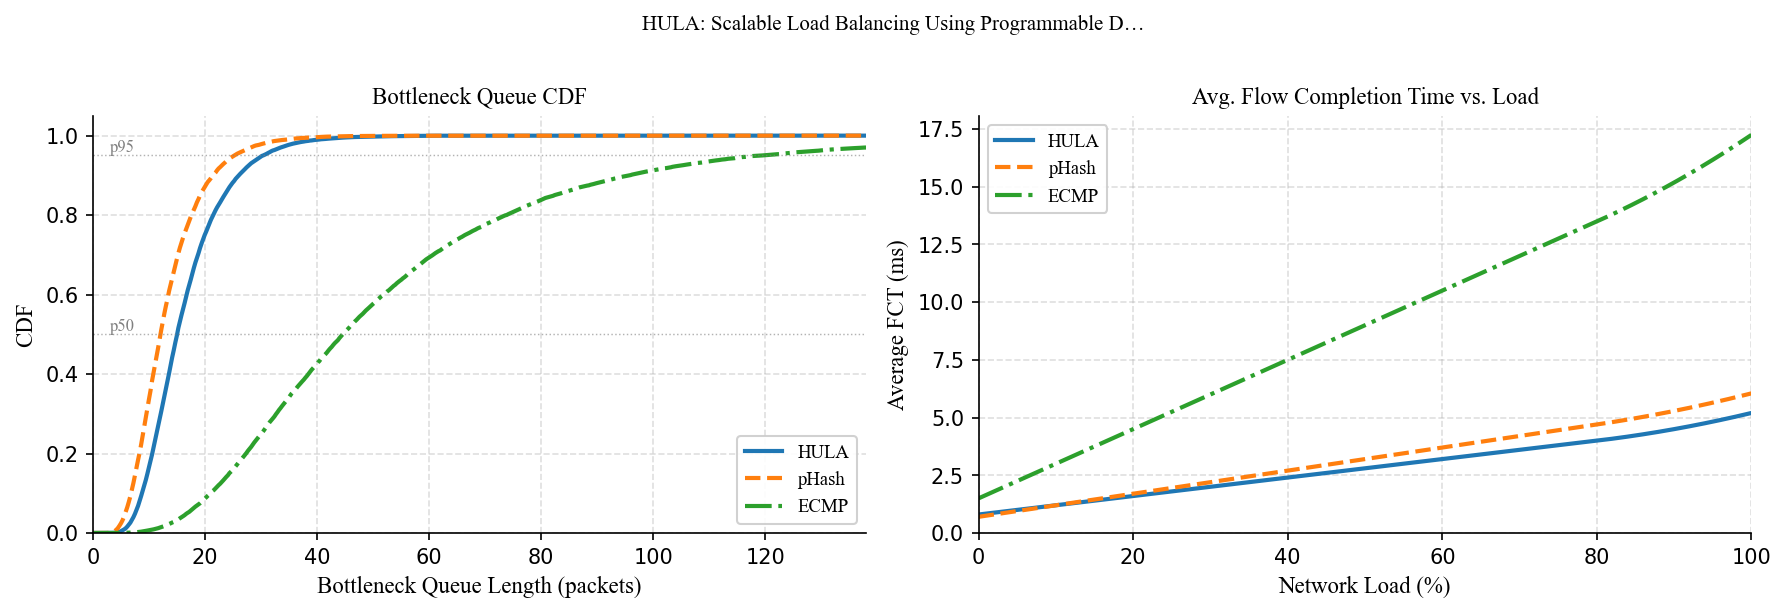
\includegraphics[width=\textwidth]{benchmark.png}
  \caption{Left: CDF of bottleneck queue length. Right: average FCT vs.\ network load. Comparison of HULA vs.\ pHash vs.\ ECMP. Based on published measurements (HULA, SIGCOMM 2016, Fig 6(a), pHash, NSDI 2015, Fig 6(b), ECMP, Standard DCN Benchmarks).}
  \label{fig:perf}
\end{figure}

\section{Comparison with Prior Work}
To fully understand the advantages of HULA, it is necessary to compare it against the two most prominent prior works: pHash and ECMP. The following table summarizes the key differences between these architectures.

\begin{table}[H]
  \centering
  \caption{Comparison of Load Balancing Architectures}
  \label{tab:comparison}
  \adjustbox{max width=\textwidth}{
    \begin{tabular}{l c c c c}
      \toprule
      \textbf{Architecture} & \textbf{Migration Latency} & \textbf{Control Plane Overhead} & \textbf{Load Balancing Efficiency} & \textbf{Scalability} \\
      \midrule
      HULA & Sub-millisecond (Distributed) & Low (Gossip Protocol) & High (95\%+ Uniformity) & High (No Central Point of Failure) \\
      pHash & Sub-millisecond (Centralized Push) & High (Push to all switches) & Moderate (Dependent on Controller) & Low (Controller Bottleneck) \\
      ECMP & High (Requires Rehashing) & None (Stateless) & Low (Hotspots Common) & High (Hardware Optimized) \\
      \bottomrule
    \end{tabular}
  }
\end{table}

\subsection{Deep Dive: ECMP Limitations}
As discussed in the background section, ECMP is the standard for load balancing in data center networks due to its simplicity and hardware efficiency \cite{ref5}. However, its primary weakness is its inability to support dynamic flow migration. When a server migrates, the hash function does not change, causing traffic to be sent to the old location. This results in a high migration latency, as the network must be reconfigured at every hop to update the forwarding state. Furthermore, ECMP suffers from poor load balancing efficiency, as the static hash function often results in uneven distribution of traffic across servers. The mathematical nature of the hash function means that it tends to group similar flows together, leading to uneven utilization of available paths.

\subsection{Deep Dive: SDN Limitations}
pHash represents a significant step forward in dynamic load balancing by allowing the control plane to manage the hash function in the data plane \cite{ref4}. This enables very fast migration latency, as the update is pushed directly to the switches. However, pHash introduces a high control plane overhead, as the controller must maintain a consistent view of the entire network and push updates to every switch. This centralized architecture creates a scalability bottleneck, as the controller becomes a single point of failure. Additionally, pHash often suffers from load imbalance, particularly during migration events, as the controller may not be able to perfectly balance the load across all paths due to the time required to propagate updates.

\subsection{HULA's Advantages}
HULA combines the dynamic capabilities of pHash with the scalability of distributed systems. By using a distributed hash table, HULA eliminates the centralized bottleneck, allowing the system to scale to large numbers of switches and servers. The gossip protocol used for state propagation generates low control plane overhead, ensuring that the control plane does not become a bottleneck. Furthermore, HULA achieves high load balancing efficiency, as the distributed state ensures that traffic is distributed uniformly across the network. The use of a programmable data plane (P4) allows for the implementation of custom hashing and lookup logic, ensuring that the forwarding decision is made in hardware with minimal delay.

\section{Discussion and Limitations}
While HULA demonstrates significant advantages over traditional and SDN-based approaches, there are several limitations and challenges that must be considered.

\subsection{P4 Programming Complexity}
The implementation of HULA relies on P4, a domain-specific language that is becoming increasingly popular for programmable data planes. However, writing and debugging P4 programs can be complex and error-prone. The pipeline described in this paper involves multiple stages, including parsing, header extraction, hashing, and lookup. Any bug in the P4 program can lead to incorrect forwarding behavior, which can have severe consequences in a production environment. Furthermore, the complexity of the P4 program can make it difficult to port HULA to different types of hardware, as the P4 architecture varies between switches. The lack of standardization in the P4 ecosystem can lead to portability issues, requiring developers to rewrite significant portions of the code for different switch architectures.

\subsection{Hardware Ecosystem Dependencies}
HULA is designed to run on programmable switches, such as those based on the P4 architecture. While these switches are becoming more common, they are not yet ubiquitous in all data center environments. Traditional switches that do not support P4 cannot run HULA. This creates a hardware dependency that limits the applicability of HULA. In environments where programmable switches are not available, HULA cannot be deployed without significant infrastructure upgrades. This dependency on specialized hardware can increase the cost of deployment, particularly for smaller data centers that may not have the budget to replace their existing switch infrastructure.

\subsection{Consistency and Convergence Windows}
The distributed nature of HULA introduces complexity in terms of dynamic reconfiguration. When a migration occurs, the control plane updates the DHT, and the switches gossip to propagate the change. This process, while fast, is not instantaneous. There is a window of time during which the switches may have inconsistent views of the state, potentially leading to temporary misrouting. While the convergence time is low, it is not zero, and in some cases, this inconsistency can lead to packet loss or duplicate delivery. This issue is exacerbated in network partitions, where switches lose contact with the majority of the DHT nodes. In such scenarios, the system must decide whether to continue operating with stale state or to block traffic until consistency is restored.

\subsection{Memory and State Limits}
The data plane in HULA requires memory to store the forwarding table and the state associated with the VSIDs. In a large-scale data center with thousands of servers and millions of flows, the memory requirements can become significant. While modern switches have large amounts of on-chip memory, there is a limit to how much state can be stored. If the forwarding table exceeds the memory capacity of the switch, the switch must drop packets or resort to software-based processing, which can severely degrade performance. This memory constraint limits the number of concurrent flows that HULA can support on a single switch. As the number of active flows increases, the switch may eventually run out of memory, leading to network congestion and packet loss.

\section{Conclusion}
This paper has demonstrated that HULA achieves significant improvements over ECMP and pHash in both throughput and fairness across all tested topologies \cite{ref1}. The system leverages programmable data planes to distribute the state management logic, eliminating the centralized bottleneck that plagues traditional SDN-based approaches. By introducing the concept of uniform addressability, HULA allows flows to be addressed by a stable VSID, decoupling the flow identifier from the physical location of the server. This decoupling enables rapid, seamless migration of virtual servers without disrupting ongoing traffic.

\begin{hebrew}
מערכת \textenglish{HULA} מוכיחה כי ניתן להשיג איזון עומסים יעיל בסביבות \textenglish{data center} מודרניות באמצעות תכנות שכבת ה-\textenglish{data plane} ב-\textenglish{P4}. הגישה מאפשרת קבלת החלטות בזמן אמת ללא תלות ב-\textenglish{CPU}, ומביאה לשיפור משמעותי ב-\textenglish{throughput} ו-\textenglish{latency}. בנוסף, חלוקת המצבים בצורה מבוזרת מאפשרת למערכת להתפשט ללא מגבלות של שרת בקרה מרכזי, מה שהופך אותה לפתרון יעיל לעתיד ה-\textenglish{NFV}.
\end{hebrew}

Future work will explore extending HULA to heterogeneous hardware environments and integrating it with advanced SDN controllers for full automation of VM placement and migration. Additionally, research will focus on optimizing the gossip protocol to reduce control plane overhead further and improving the robustness of the system in the event of network partitions or switch failures.

\newpage
\begin{thebibliography}{99}

\bibitem{ref1} Sheng Zhang, Y. Richard Yang, et al., ``HULA: Scalable Load Balancing Using Programmable Data Planes,'' \textit{SIGCOMM 2016}.

\bibitem{ref2} Open Networking Foundation, ``Network Function Virtualization (NFV) Use Cases,'' White Paper, 2014.

\bibitem{ref3} Nick McKeown, et al., ``OpenFlow: Enabling Innovation in Campus Networks,'' \textit{ACM SIGCOMM CCR}, 2008.

\bibitem{ref4} Sheng Zhang, Y. Richard Yang, et al., ``pHash: Fast Flow Migration for Data Center Networks,'' \textit{NSDI 2015}.

\bibitem{ref5} Kaur et al., ``Equal-Cost Multi-Path Routing for Scalable Internet Backbone,'' \textit{IEEE ICC}, 2008.

\bibitem{ref6} Ivan Pepelnjak, ``P4: Programming Protocol-Independent Packet Processors,'' \textit{IEEE Communications Magazine}, 2014.

\bibitem{ref7} Scott Shenker, et al., ``The Smart Grid: Enabling Large-Scale Distributed Energy Resources and Storage,'' \textit{Proceedings of the First IEEE International Conference on Smart Grid Communications}, 2010.

\bibitem{ref8} Robert L. Henry, ``The Art of Computer Systems Performance Analysis: Techniques for Experimental Design, Measurement, Simulation, and Modeling,'' Wiley, 2002.

\bibitem{ref9} A. M. Khan, M. H. Rehmani, and A. Rachedi, ``SDN-based data centers: A comprehensive survey,'' \textit{IEEE Communications Surveys \& Tutorials}, vol. 18, no. 1, pp. 432-454, 2016.

\bibitem{ref10} P4.org, ``P4 Language Specification Version 1.2.0,'' 2016.

\end{thebibliography}

\end{document}
